Testiranja su obavaljena na računalu s procesorom Intel Core i7 920 @ 2.66 GHz, s 6 GB RAM memorije i na operacijskom sustavu Windows 7. Razlog zašto testiranja nisu bila obaljena na Biolinuxu (ili nekoj drugoj Linux distribuciji) je taj što se Biolinux, na računalu koje se je koristilo za testiranja, pokreće u virtualnom stroju, pa je upitno kako bi to utjecalo na performanse izvođenja samog programa.

Za obavljanje ovih testiranja korištena su tri tipa tekstualnih datoteka. Prvi tip tekstualnih datoteka se je sastojao od nizova nukleotida i dodatnih znakova koji se još mogu pojaviti u takvim nizovima. Drugi tip takstualnih datoteka sastojao se je od nizova znakova koji predstavljaju proteine. Posljednji tip tekstualnih datoteka koje su korištene sastojale su se od nizova slučajno generiranih znakova iz osnovnog ASCII skupa znakova. Prvi i drugi tip datoteka su preuzeti sa [referenca na pizza i chilli] te su ponešto prilagođene za obavljanje testiranja. Treći tip datoteka je bio generiran uz pomoć posebnog programa.

U ovom poglavlju pogledat ćemo performanse koje pruža implementirani FM-Index i to u tri kategorije: brzina izgradnje, brzina obavljanja \textit{count} upita i memorijska potrošnja.

\section{Vrijeme izgradnje FM-Indexa}
Pogledajmo prvo performanse izgradnje FM-indexa. Ovo je možda i jedan od najbitnijih faktora prilikom ocjene koliko je neka implementacija dobra, pošto je izgradnja samog indeksa računalno veoma zahtjevna operacija. Kako bi rezultati koji će biti prikazani u ovom poglavlju bili što relevantniji, vrijednosti koje su prikazane u tablicama izračunate su kao prosjek od deset izgradnji FM-indeksa za svaku pojedinu veličinu datoteka. Osim toga, prilikom provođenja ovih eksperimenata nije bio pokrenut profiler, jer on dodatno usporava izvođenje programa, stoga su mjerenja za memorijsku potrošnju obavljena zasebno. Eksperimenti su ovaljnei za svaki tip datoteke koji bio ranije spomenut i to za 9 različith veličina takvih datoteka, od manjih (1MB), pa sve do većih (500MB). Osim toga, posebno su izdvojena vremena izgradnje BWT transformacije i Wavelet stabla, koji ipak sačinjavaju glavne građevne blokove FM-Indexa, pa je iz tog razloga dobro vidjeti koliko se mijenja i vrijeme izgradnje ovih struktura s promjenom veličine ulazne datoteke.

Pogledajmo prvo rezultate koji su dobiveni za datoteke koje su sadržavale nizove nukleotida. Tablica \ref{tbl:tablNukleotidi} prikazuje vremena izgradnje FM-Indexa nad tipom datoteka koje sadrže nukleotide. Dodatno su iscrtana tri grafa koji prikazuju kako se brzina izgradnje FM-Indeksa i nekih njegovi djelova ponaša s povečanjem nizova nad kojima se te strukture izgrađuju. Tako graf \ref{} prikazuje ovisnost vremena izgradnje FM-Indexa u odnosu na veličinu ulaznog niza, graf \ref{} prikazuje ovisnost algoritam izgradnje sufisknog stavla u odnosu na veličinu ulaznaog niza i graf ref{} izgradnju Wavelet stabla u ovisnosti na veličinu ulaznog niza.

TABLICA NUKLEOTIDI


\begin{table}[h]
\caption{Testiranje na nizu nukleotida}
\label{tbl:tablNukleotidi}
\centering
\begin{tabular}{c|c|c|c|}
\cline{2-4}
      	    					 & \multicolumn{3}{c|}{vrijeme izgradnje (s)}  \\ \hline
\multicolumn{1}{ |c| } {veličina (MB)} &	 BWT 	& wavelet stablo & FM indeks  \\ \hline 
\multicolumn{1}{ |c| } {   1    } 		& 	0.4694	&	0.1431	&	0.6954	\\ \hline
\multicolumn{1}{ |c| } {   2    } 		& 	0.6427	&	0.1881	&	0.9581	\\ \hline
\multicolumn{1}{ |c| } {   5    } 		& 	1.4017	&	0.3137	&	1.9724	\\ \hline
\multicolumn{1}{ |c| } {   10    } 	&	2.9828	&	0.5214	&	3.9738	\\ \hline
\multicolumn{1}{ |c| } {   20    } 	&	6.7284	&	0.9268	&	8.5542	\\ \hline
\multicolumn{1}{ |c| } {   50    } 	&	21.1193	&	3.5455	&	27.0914	\\ \hline
\multicolumn{1}{ |c| } {   100    } 	&	46.4439	&	6.2703	&	57.6676	\\ \hline
\multicolumn{1}{ |c| } {   200    } 	&	101.1712	&	11.9061	&	122.9448	\\ \hline
\multicolumn{1}{ |c| } {   500    } 	&	284.38207	&	29.0901	&	338.5938	\\ \hline
\end{tabular}
\end{table}






GRAF FMINDEX
GRAF BWT
GRAF WAVELET


Ukoliko malo proučimo podatke iz tablice i grafova, možemo vidjeti kako je složenost izgradnje indeksa linearno ovisna o veličini ulaznog niza. To je svojstvo koje smo i željeli postići, ondnosno htjeli smo da nam je složenost izgradnje indeksa linearna. No svejedno vidimo kako je složenost izgradnje FM-Indexa za veće nizove veoma zahtjevan i dugotrajan proces te da za veće ulazne nizove može potrajati i po nekoliko minuta.

U tablici \ref{tbl:tablProteini} prikazani su rezultati koji su dobiveni za datoteke koje su sadržavale proteinske nizove. Graf \ref{} prikazuje ovisnost trajanje izgradnje FM-Indeksa o veličini ulaznog niza (odnosno ulazne datoteke), dok slike \ref{} i \re{} prikazuju ovisnost izračunavanja BWT transformacije i izgradnje Wavelet stabla respektivno, u ovisnosti o veličini ulaznog niza.


\begin{table}[h]
\caption{Testiranje na proteinima}
\label{tbl:tablProteini}
\centering
\begin{tabular}{c|c|c|c|}
\cline{2-4}
      	    					 & \multicolumn{3}{c|}{vrijeme izgradnje (s)}  \\ \hline
\multicolumn{1}{ |c| } {veličina (MB)} &	 BWT 	& wavelet stablo & FM indeks  \\ \hline 
\multicolumn{1}{ |c| } {   1    } 		& 	0.4547	&	0.366	&	0.9295	\\ \hline
\multicolumn{1}{ |c| } {   2    } 		& 	0.6815	&	0.4119	&	1.2776	\\ \hline
\multicolumn{1}{ |c| } {   5    } 		& 	1.5011	&	0.5886	&	2.5025	\\ \hline
\multicolumn{1}{ |c| } {   10    } 	&	3.2401	&	0.8957	&	4.9289	\\ \hline
\multicolumn{1}{ |c| } {   20    } 	&	7.392		&	1.4896	&	10.4347	\\ \hline
\multicolumn{1}{ |c| } {   50    } 	&	24.1723	&	4.61334	&	32.6025	\\ \hline
\multicolumn{1}{ |c| } {   100    } 	&	52.6474	&	7.7732	&	67.9625	\\ \hline
\multicolumn{1}{ |c| } {   200    } 	&	112.8949	&	13.9333	&	142.1054	\\ \hline
\multicolumn{1}{ |c| } {   500    } 	&	315.5526	&	32.8476	&	386.6631	\\ \hline
\end{tabular}
\end{table}




Konačno, u tablici \ref{tbl:tablRand} je prikazana i ovisnost izgradnje FM-Indexa o veličini ulaznog niza za treću vrstu datoteka. Ovisnost izgradnje FM-Indexa, provođenja BWT transformacije, kao i izgradnju Wavelet stabla, u odnosu na veličinu ulaznog niza prikazuju grafovi \ref{}, \ref{} i \ref{}, respektivno.


\begin{table}[h]
\caption{Testiranje na rand}
\label{tbl:tablRand}
\centering
\begin{tabular}{c|c|c|c|}
\cline{2-4}
      	    					 & \multicolumn{3}{c|}{vrijeme izgradnje (s)}  \\ \hline
\multicolumn{1}{ |c| } {veličina (MB)} & 	BWT 		& wavelet stablo & FM indeks  \\ \hline  
\multicolumn{1}{ |c| } {   1    } 		& 	0.4795	&	1.2554	&	1.9021	\\ \hline
\multicolumn{1}{ |c| } {   2    } 		& 	0.772	&	1.3382	&	2.4216	\\ \hline
\multicolumn{1}{ |c| } {   5    } 		& 	1.8199	&	1.789	&	4.34387	\\ \hline
\multicolumn{1}{ |c| } {   10    } 	&	4.2868	&	2.579	&	8.3161	\\ \hline
\multicolumn{1}{ |c| } {   20    } 	&	10.2298	&	4.061	&	17.1314	\\ \hline
\multicolumn{1}{ |c| } {   50    } 	&	31.4606	&	8.3703	&	46.9771	\\ \hline
\multicolumn{1}{ |c| } {   100    } 	&	72.435	&	15.4384	&	103.1664	\\ \hline
\multicolumn{1}{ |c| } {   200    } 	&	163.362	&	29.5337	&	223.3576	\\ \hline
\multicolumn{1}{ |c| } {   500    } 	&	447.88	&	66.3437	&	588.4351	\\ \hline
\end{tabular}
\end{table}


\begin{figure}[h]
   \centering
       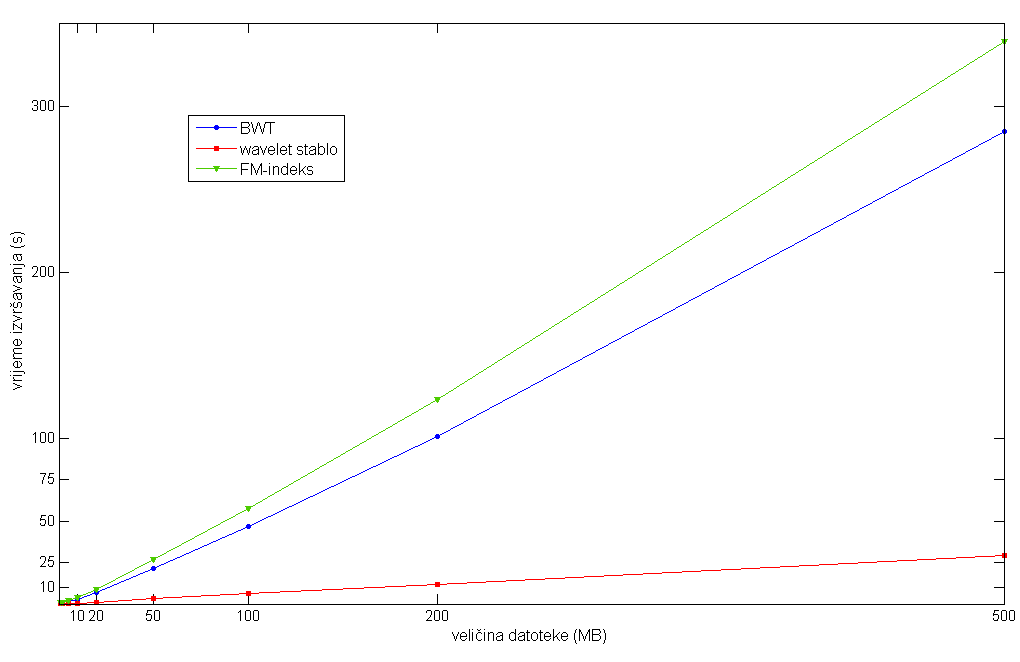
\includegraphics[width=\textwidth]{./pictures/test_nukl.png}
 \caption{Vremenska ovisnost trajanja algoritama o veličini datoteke koja sadrži nukleotide}
 \label{fig:test_nukl}
\end{figure}

\begin{figure}[h]
   \centering
       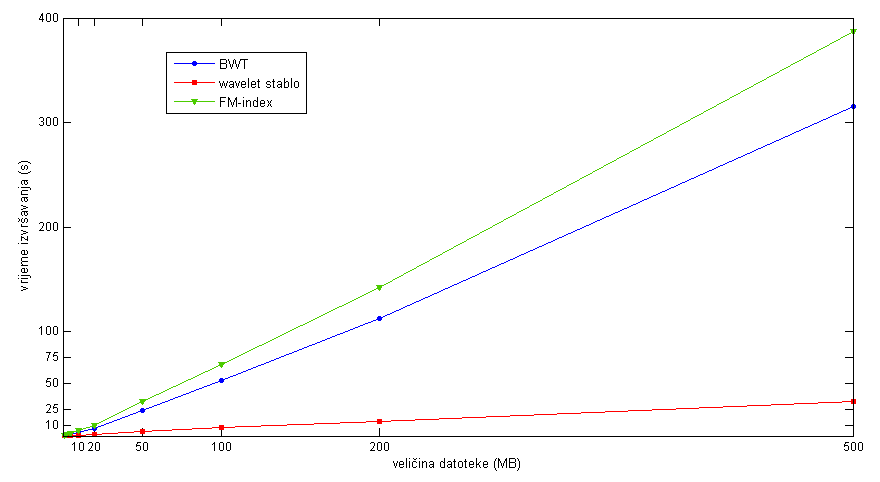
\includegraphics[width=\textwidth]{./pictures/test_proteini.png}
 \caption{Vremenska ovisnost trajanja algoritama o veličini datoteke koja sadrži proteine}
 \label{fig:test_proteini}
\end{figure}

\begin{figure}[h]
   \centering
       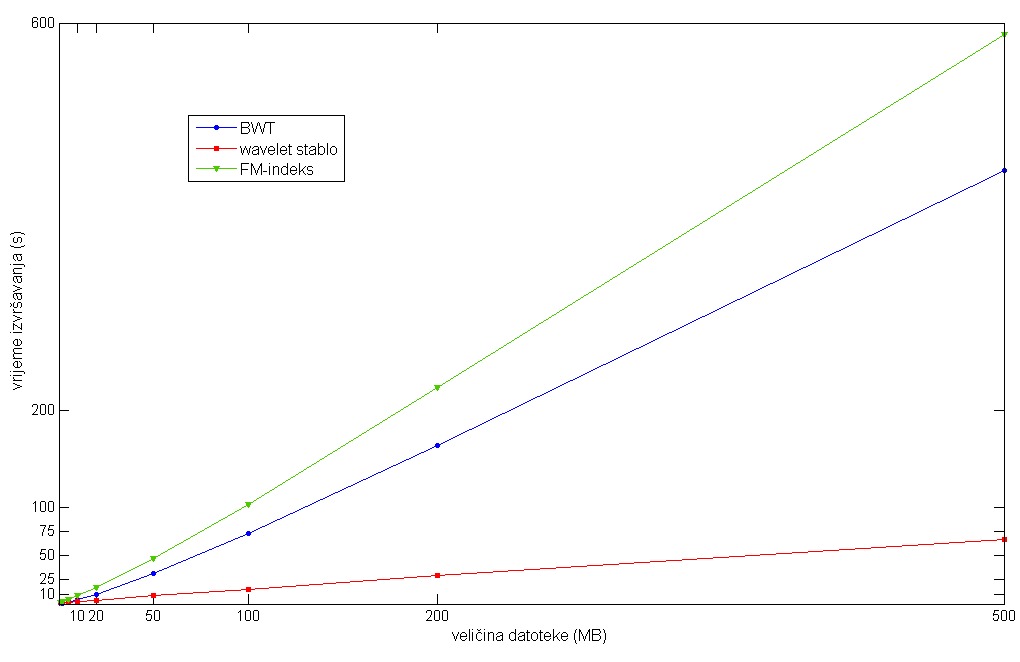
\includegraphics[width=\textwidth]{./pictures/test_ascii.png}
 \caption{Vremenska ovisnost trajanja algoritama o veličini datoteke koja sadrži ASCII znakove}
 \label{fig:test_ascii}
\end{figure}

\begin{figure}[h]
   \centering
       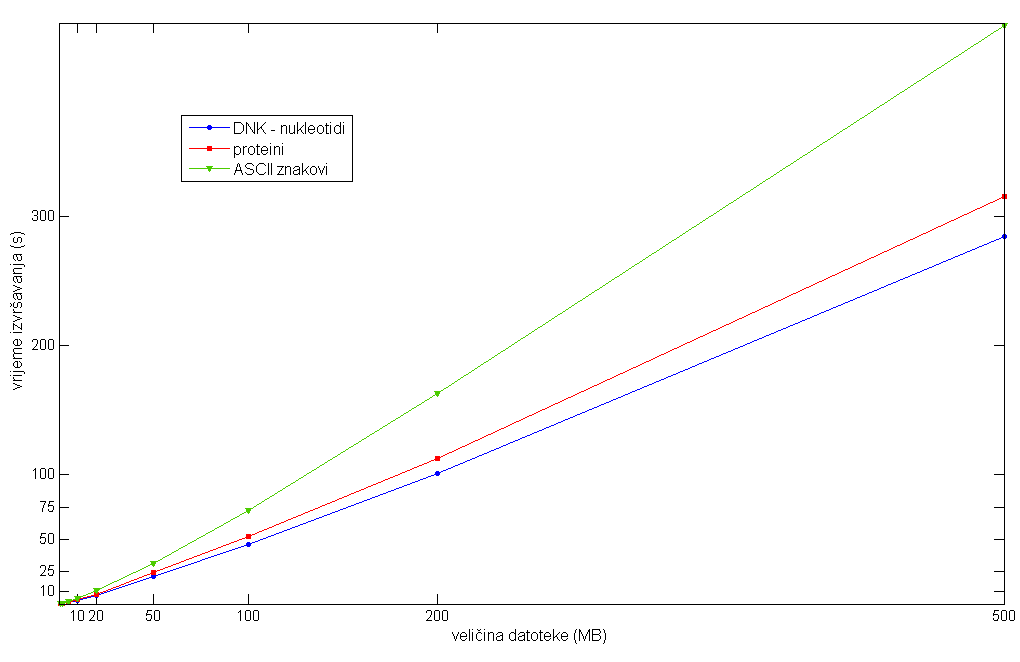
\includegraphics[width=\textwidth]{./pictures/test_bwt.png}
 \caption{Vremenska ovisnost trajanja BWT algoritma o veličini datoteke određenog tipa}
 \label{fig:test_bwt}
\end{figure}

\begin{figure}[h]
   \centering
       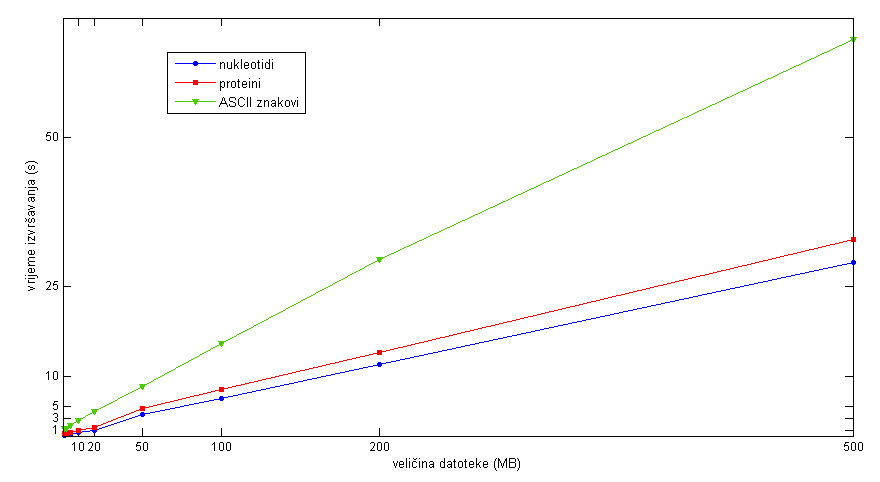
\includegraphics[width=\textwidth]{./pictures/test_wavelet.png}
 \caption{Vremenska ovisnost trajanja stvaranja wavelet stabla o veličini datoteke određenog tipa}
 \label{fig:test_wavelet}
\end{figure}

\begin{figure}[h]
   \centering
       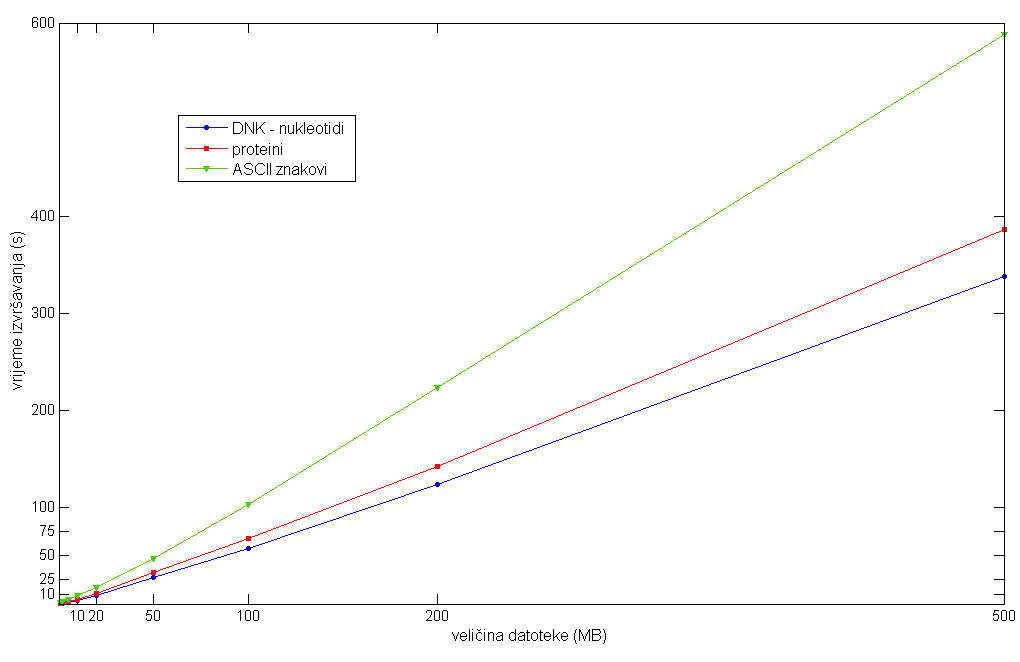
\includegraphics[width=\textwidth]{./pictures/test_fm.png}
 \caption{Vremenska ovisnost trajanja stvaranja FM-indexa o veličini datoteke određenog tipa}
 \label{fig:test_fm}
\end{figure}




\section{Vrijeme obavljanja \textit{count} upita}

Drugi važan parametar pomoću kojeg se može ocijeniti uspješnost implementacije FM-Indeksa jest obavljanje \textit{count} upita nad izgrađenim nizom. 

\begin{figure}[h]
   \centering
       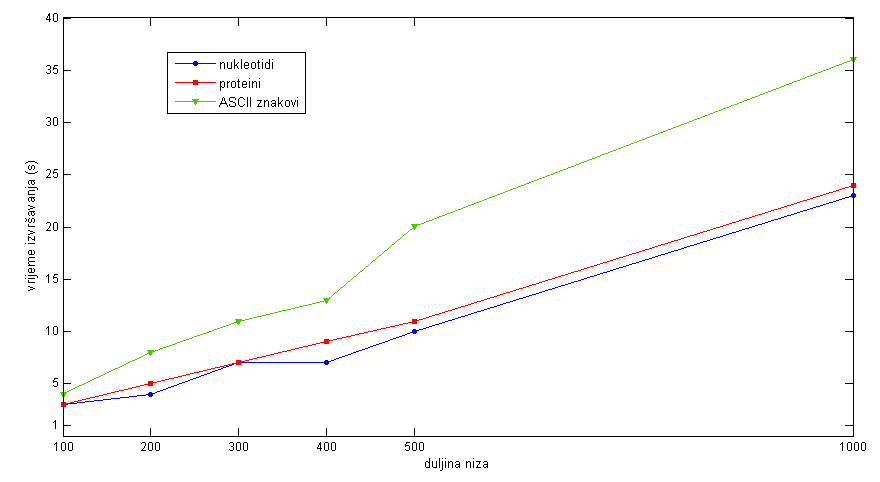
\includegraphics[width=\textwidth]{./pictures/test_count.png}
 \caption{Vremenska ovisnost izvršavanja \emph{count} algoritma o veličini niza koji se prebrojava}
 \label{fig:test_count}
\end{figure}



\begin{table}[h]
\caption{Count upit nad nizom nukleotida}
\label{tbl:tablCountNukl}
\centering
\begin{tabular}{c|c|c|c|c|c|c|}
\cline{2-7}
							& \multicolumn{6}{|c|}{trajanje prebrojavanja (s)}  \\ \cline{2-7}  
      	    					 	& \multicolumn{6}{c|}{duljina traženog niza}  \\ \hline
\multicolumn{1}{ |c| } {veličina (MB)} & 100 & 200 & 300 & 400 & 500 & 1000	\\ \hline  
\multicolumn{1}{ |c| } {   1    } 		& 2 	& 3 	 & 5	    & 7	 & 8	 & 17		\\ \hline
\multicolumn{1}{ |c| } {   2    } 		& 2 	& 4	 & 5 	    & 7 	 & 7	 & 17 	\\ \hline
\multicolumn{1}{ |c| } {   5    } 		& 2 	& 3	 & 5	    & 7	 & 7	 & 16		\\ \hline
\multicolumn{1}{ |c| } {   10    } 	& 2 	& 3	 & 5	    & 7	 & 8	 & 16		\\ \hline
\multicolumn{1}{ |c| } {   20    } 	& 1	& 4	 & 5	    & 7	 & 8	 & 16		\\ \hline
\multicolumn{1}{ |c| } {   50    } 	& 2 	& 5	 & 7	    & 8	 & 10	 & 22		\\ \hline
\multicolumn{1}{ |c| } {   100    }	& 2 	& 4	 & 7	    & 8	 & 10 & 22		\\ \hline  
\multicolumn{1}{ |c| } {   200    }	& 2 	& 4	 & 7	    & 9	 & 9	 & 22		\\ \hline	
\multicolumn{1}{ |c| } {   500    } 	& 3 	& 4	 & 7	    & 7 	& 10	 & 23		\\ \hline
\end{tabular}
\end{table}



\begin{table}[h]
\caption{Count upit nad proteinima}
\label{tbl:tablCountProt}
\centering
\begin{tabular}{c|c|c|c|c|c|c|}
\cline{2-7}
							& \multicolumn{6}{|c|}{trajanje prebrojavanja (s)}  \\ \cline{2-7}  
      	    					 	& \multicolumn{6}{c|}{duljina traženog niza}  \\ \hline
\multicolumn{1}{ |c| } {veličina (MB)} & 100 & 200 & 300 & 400 & 500 & 1000	\\ \hline  
\multicolumn{1}{ |c| } {   1    } 		& 3 	& 5    & 8	    & 9	& 9	 & 25		\\ \hline
\multicolumn{1}{ |c| } {   2    } 		& 3 	& 5	 & 8	    & 8 	& 10	 & 24		\\ \hline
\multicolumn{1}{ |c| } {   5    } 		& 3 	& 5	 & 7	    & 9	& 10	 & 23		\\ \hline
\multicolumn{1}{ |c| } {   10    } 	& 2 	& 5	 & 7	    & 8	& 10	 & 23		\\ \hline
\multicolumn{1}{ |c| } {   20    } 	& 2	& 5	 & 8	    & 9	& 11	 & 24		\\ \hline
\multicolumn{1}{ |c| } {   50    } 	& 2 	& 6	 & 8	    & 9	& 11	 & 26		\\ \hline
\multicolumn{1}{ |c| } {   100    }	& 2 	& 5	 & 9 	    & 9 	& 12	 & 24		\\ \hline  
\multicolumn{1}{ |c| } {   200    }	& 3 	& 5	 & 8	    & 9 	& 11	 & 25		\\ \hline	
\multicolumn{1}{ |c| } {   500    } 	& 3 	& 5	 & 7	    & 9	& 11	 & 24		\\ \hline
\end{tabular}
\end{table}


\begin{table}[h]
\caption{Count upit nad rand}
\label{tbl:tablCountRand}
\centering
\begin{tabular}{c|c|c|c|c|c|c|}
\cline{2-7}
							& \multicolumn{6}{|c|}{trajanje prebrojavanja (s)}  \\ \cline{2-7}  
      	    					 	& \multicolumn{6}{c|}{duljina traženog niza}  \\ \hline
\multicolumn{1}{ |c| } {veličina (MB)} & 100 & 200 & 300 & 400 & 500 & 1000	\\ \hline 
\multicolumn{1}{ |c| } {   1    } 		& 3 	& 8 	 & 11	    & 13	& 18	 & 34		\\ \hline
\multicolumn{1}{ |c| } {   2    } 		& 4 	& 7	 & 11	    & 12 	& 18	 & 33		\\ \hline
\multicolumn{1}{ |c| } {   5    } 		& 4 	& 7	 & 10	    & 12	& 19	 & 34		\\ \hline
\multicolumn{1}{ |c| } {   10    } 	& 4 	& 8	 & 10	    & 13	& 19	 & 35		\\ \hline
\multicolumn{1}{ |c| } {   20    } 	& 4	& 8	 & 10	    & 12	& 19	 & 35		\\ \hline
\multicolumn{1}{ |c| } {   50    } 	& 4 	& 8	 & 11	    & 13 	& 19	 & 35		\\ \hline
\multicolumn{1}{ |c| } {   100    }	& 4 	& 8	 & 11	    & 14	& 20	 & 36		\\ \hline
\multicolumn{1}{ |c| } {   200    }	& 4 	& 8	 & 11	    & 13 	& 19	 & 38		\\ \hline
\multicolumn{1}{ |c| } {   500    } 	& 4 	& 8	 & 11	    & 13 	& 20	 & 36		\\ \hline
\end{tabular}
\end{table}





\section{Memorijsko zauzeće FM-indexa}

Posljednji parametar kojeg možemo promatrati tijekom izrade FM-indeksa jest memorijsko zauzeće programa. U ovom poglavlju istaknut ćemo koliko je memorijsko zauzeće tokom izgradnje indeksa, kao i na kraju kada je indeks u potpunosti izgrađen. Osim toga, u ovom poglavlju pokazat će se kako Java virtualni stroj zauzima mnogo više memorije nego što je zaista potrebno za samo izvođenje algoritma, što predstavlja jedan veliki nedostatak. Ovdje će se razmotriti memorijska zauzeća za sve tipove datoteka, no promatrat će se samo veličine datoteka od 50MB nadalje. To je napravljeno iz razloga što i sam Java virtualni stroj sam po sebi zauzima dosta memorije, bez da je išta pokrenuto, te bi na manjim datotekama bio veći utjecaj Java virtualnog stroja nego samog algoritma i stoga rezultati ne bi bili u potpunosti relevantni. Ovako kada su mjerenja obavljena nad 


\begin{table}[h]
\caption{Memorijsko zauzeće - niz nukleotida}
\label{tbl:tablMemNukl}
\centering
\begin{tabular}{c|c|c|c|}
\cline{2-4}
      	   & \multicolumn{3}{c|}{memorijsko zauzeće (MB)}  \\ \hline
\multicolumn{1}{ |c| } {veličina (MB)} & maksimalno & pravo & konačno  \\ \hline
\multicolumn{1}{ |c| } {   50   }		&	393	&	314	&	53	\\ \hline
\multicolumn{1}{ |c| } {  100  }		&	803	&	620	&	103	\\ \hline
\multicolumn{1}{ |c| } {  200  }		&	1553	&	1230	&	201	\\ \hline
\multicolumn{1}{ |c| } {  500   } 	&	3830	&	3080	&	494	\\ \hline
\end{tabular}
\end{table}



\begin{table}[h]
\caption{Memorijsko zauzeće - protieni}
\label{tbl:tablMemProt}
\centering
\begin{tabular}{c|c|c|c|}
\cline{2-4}
      	   & \multicolumn{3}{c|}{memorijsko zauzeće (MB)}  \\ \hline
\multicolumn{1}{ |c| } {veličina (MB)} & maksimalno & pravo & konačno  \\ \hline
\multicolumn{1}{ |c| } {   50   }		&	370	&	292	&	67	\\ \hline
\multicolumn{1}{ |c| } {   100   }	&	800	&	614	&	130	\\ \hline
\multicolumn{1}{ |c| } {   200   }	&	1550	&	1230	&	254	\\ \hline
\multicolumn{1}{ |c| } {   500   }	&	4800	&	3070	&	680	\\ \hline
\end{tabular}
\end{table}


\begin{table}[h]
\caption{Memorijsko zauzeće - rand}
\label{tbl:tablMemRand}
\centering\begin{tabular}{c|c|c|c|}
\cline{2-4}
      	   & \multicolumn{3}{c|}{memorijsko zauzeće (MB)}  \\ \hline
\multicolumn{1}{ |c| } {veličina (MB)} & maksimalno & pravo & konačno  \\ \hline
\multicolumn{1}{ |c| } {   50   }		&	432	&	365	&	100	\\ \hline
\multicolumn{1}{ |c| } {   100   }	&	800	&	619	&	191	\\ \hline
\multicolumn{1}{ |c| } {   200   }	&	1558	&	1235	&	378	\\ \hline
\multicolumn{1}{ |c| } {   500   }	&	4000	&	3700	&	840	\\ \hline
\end{tabular}
\end{table}



\begin{figure}[h]
   \centering
       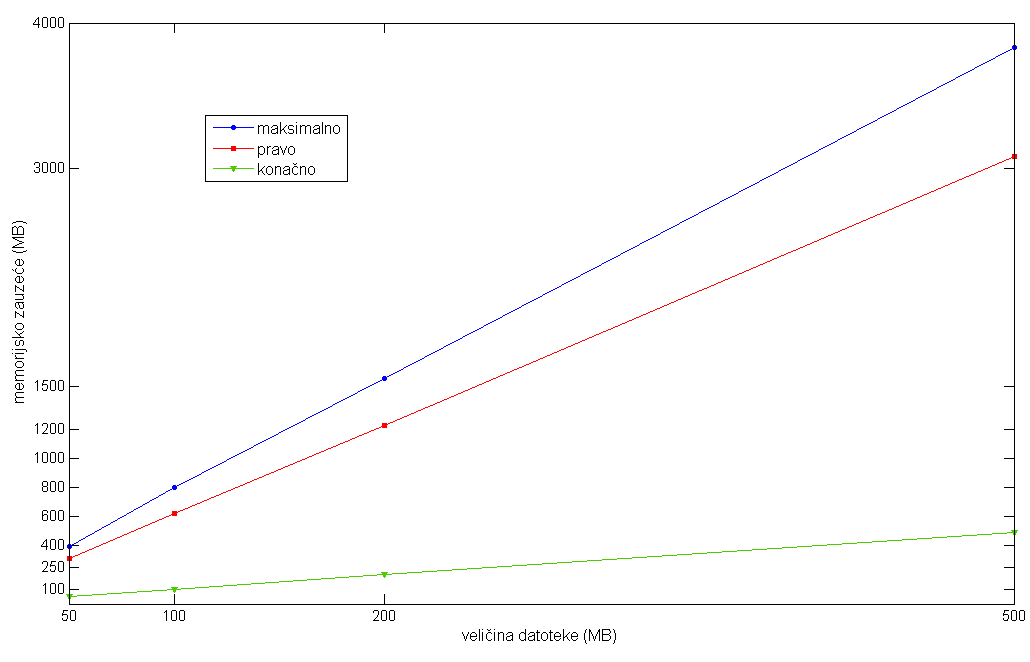
\includegraphics[width=\textwidth]{./pictures/test_mem_nukl.png}
 \caption{Memorijska ovisnost stvaranja FM-indeksa algoritama o veličini datoteke koja sadrži nukleotide}
 \label{fig:test_mem_nukl}
\end{figure}

\begin{figure}[h]
   \centering
       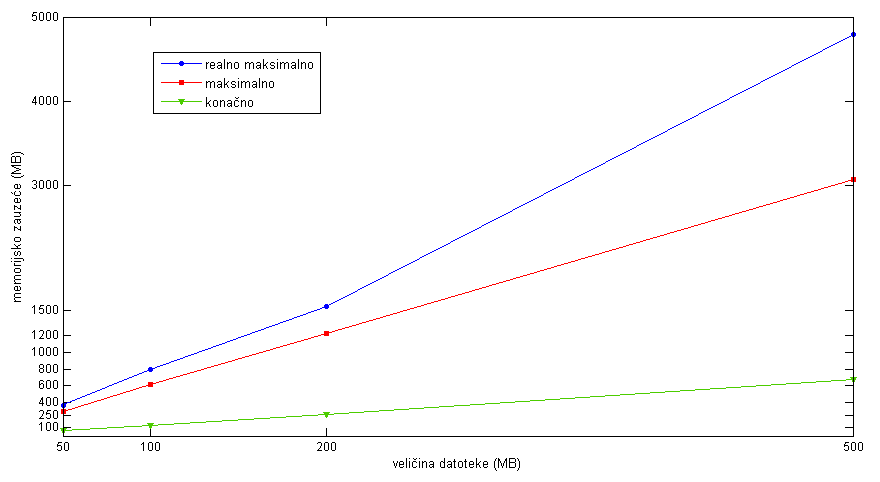
\includegraphics[width=\textwidth]{./pictures/test_mem_proteini.png}
 \caption{Memorijska ovisnost stvaranja FM-indeksa algoritama o veličini datoteke koja sadrži proteine}
 \label{fig:test_mem_proteini}
\end{figure}

\begin{figure}[h]
   \centering
       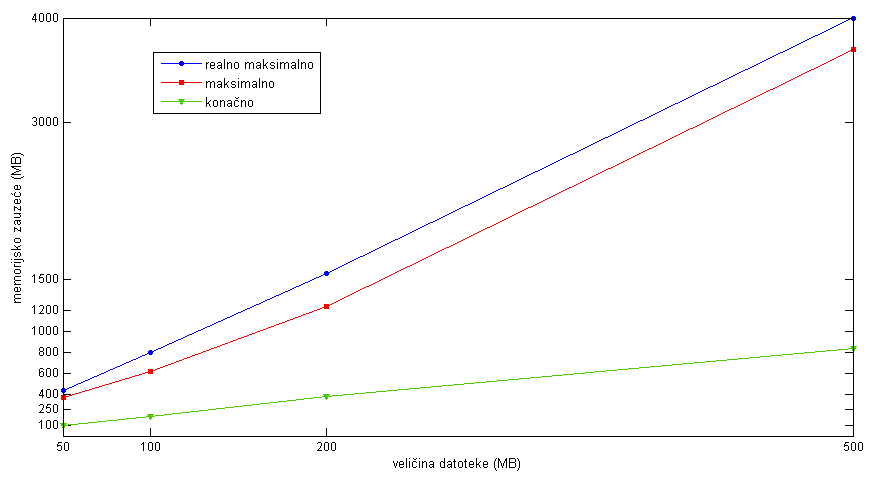
\includegraphics[width=\textwidth]{./pictures/test_mem_ascii.png}
 \caption{Memorijska ovisnost stvaranja FM-indeksa algoritama o veličini datoteke koja sadrži ASCII znakove}
 \label{fig:test_mem_ascii}
\end{figure}

\begin{figure}[h]
   \centering
       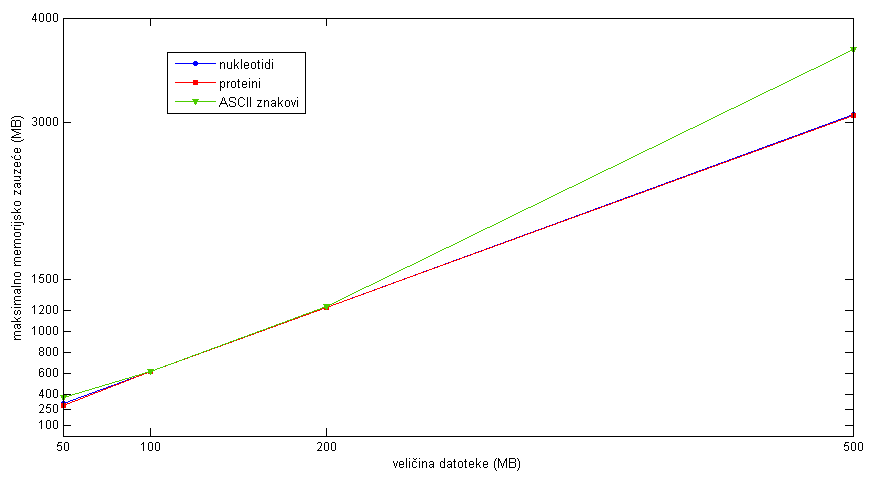
\includegraphics[width=\textwidth]{./pictures/test_mem_max.png}
 \caption{Memorijska (maksimalna) ovisnost stvaranja FM-indeksa o veličini datoteke određenog tipa}
 \label{fig:test_mem_max}
\end{figure}

\begin{figure}[h]
   \centering
       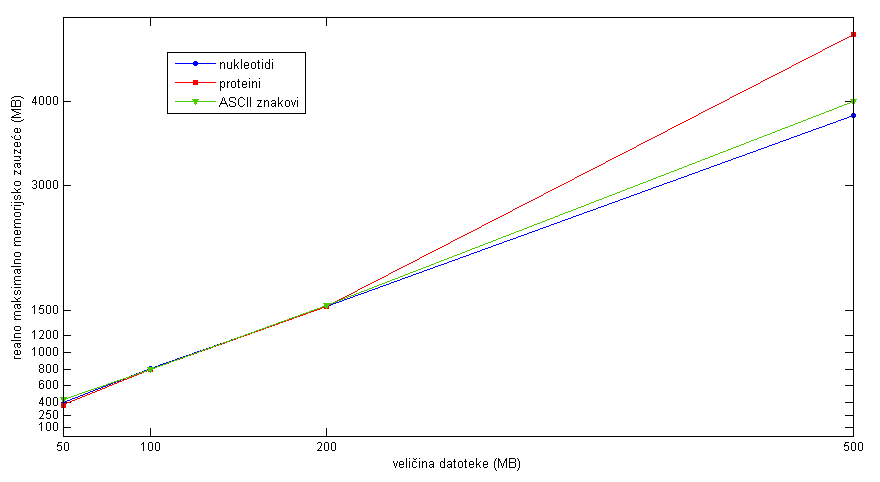
\includegraphics[width=\textwidth]{./pictures/test_mem_realmax.png}
 \caption{Memorijska (realno maksimalna) ovisnost stvaranja FM-indeksa o veličini datoteke određenog tipa}
 \label{fig:test_mem_realmax}
\end{figure}

\begin{figure}[h]
   \centering
       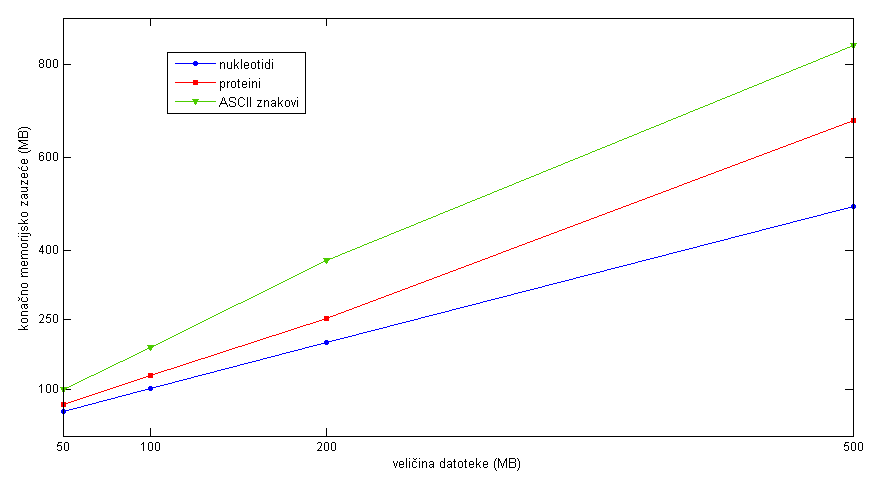
\includegraphics[width=\textwidth]{./pictures/test_mem_kon.png}
 \caption{Memorijska (konačna) ovisnost stvaranja FM-indeksa o veličini datoteke određenog tipa}
 \label{fig:test_mem_kon}
\end{figure}




Pogledajmo sada sliku \ref{profiler} koja je preuzeta iz profilera koje predstavlja memorijsko zauzeće algoritma kroz vrijeme. Plavom bojom označena je memorija koju program, odnsono algoritam stvarno koristi za spremanje struktura, dok je zelenom bojom označena slobodna memorija koju je Java virtualni stroj dodatno zauzeo. Vidimo da cijelo vrijeme Java virtualni stroj zauzima mnogo više memorije nego što mu doista treba za rad. To je ogroman nedostatak pri izradi memorijski zahtjevnih algoritama kao što je ovaj, jer Java programski jezik ne omogućuje efikasno rukovanje memorijom.

\begin{figure}[H]
   \centering
       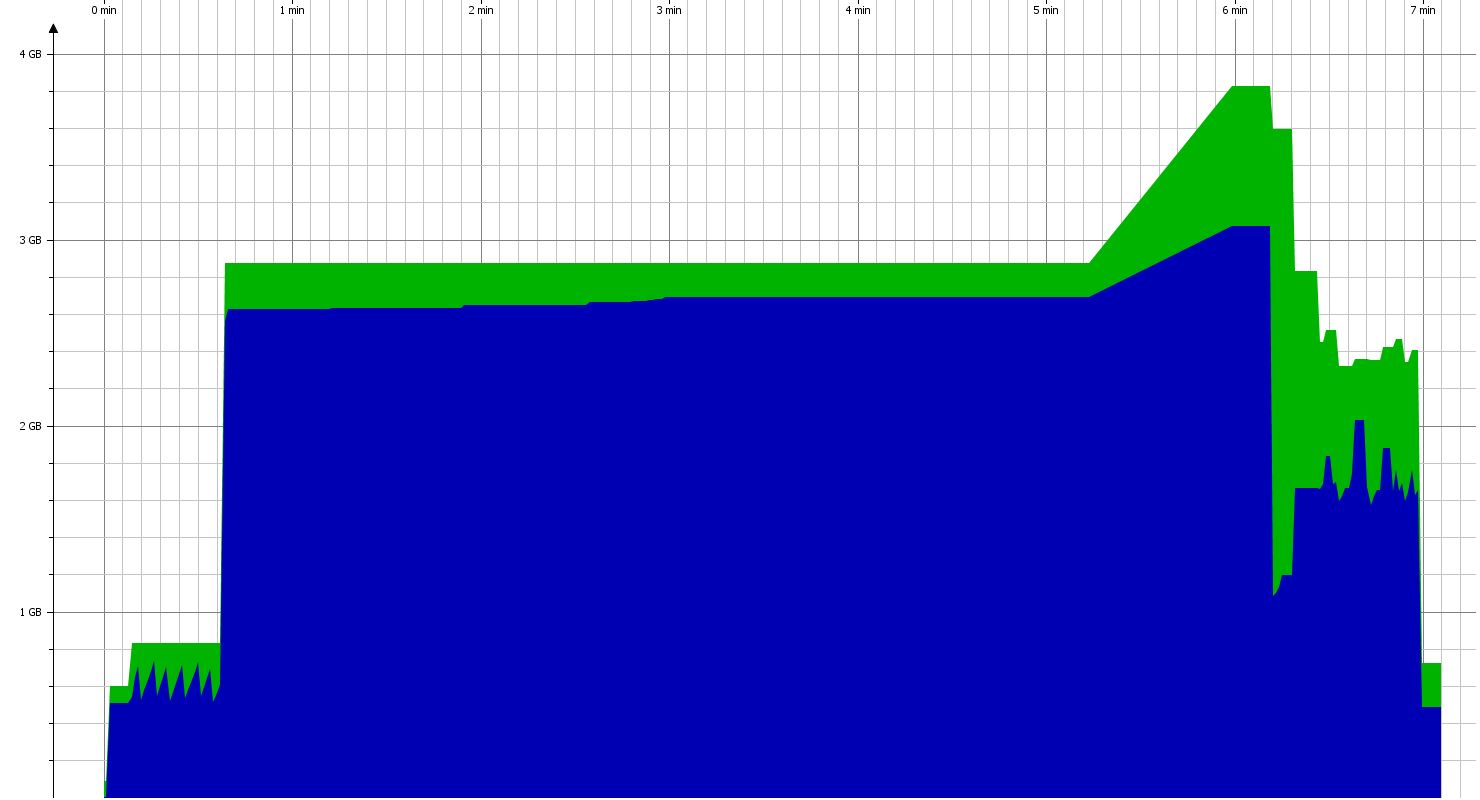
\includegraphics[width=\linewidth]{./pictures/profiler.jpg}
 \caption{Zauzeće memorije Java virtualnog stroja tijekom konstrukcije indeksa}
 \label{fig:profiler}
\end{figure}